% !TeX root = ../main.tex
\section{System Architecture}

Figure~\ref{fig:architecture} separates approved intent from base and proposed implementation state. ArchSync Core validates the model and provides the expected graph and executable rules. Guardian caches a base Observed Graph, scopes the Git diff to affected source components, incrementally constructs the head graph, and preserves source evidence. The gate compares base and head findings before deriving the pull-request decision.

\begin{figure*}[t]
  \centering
  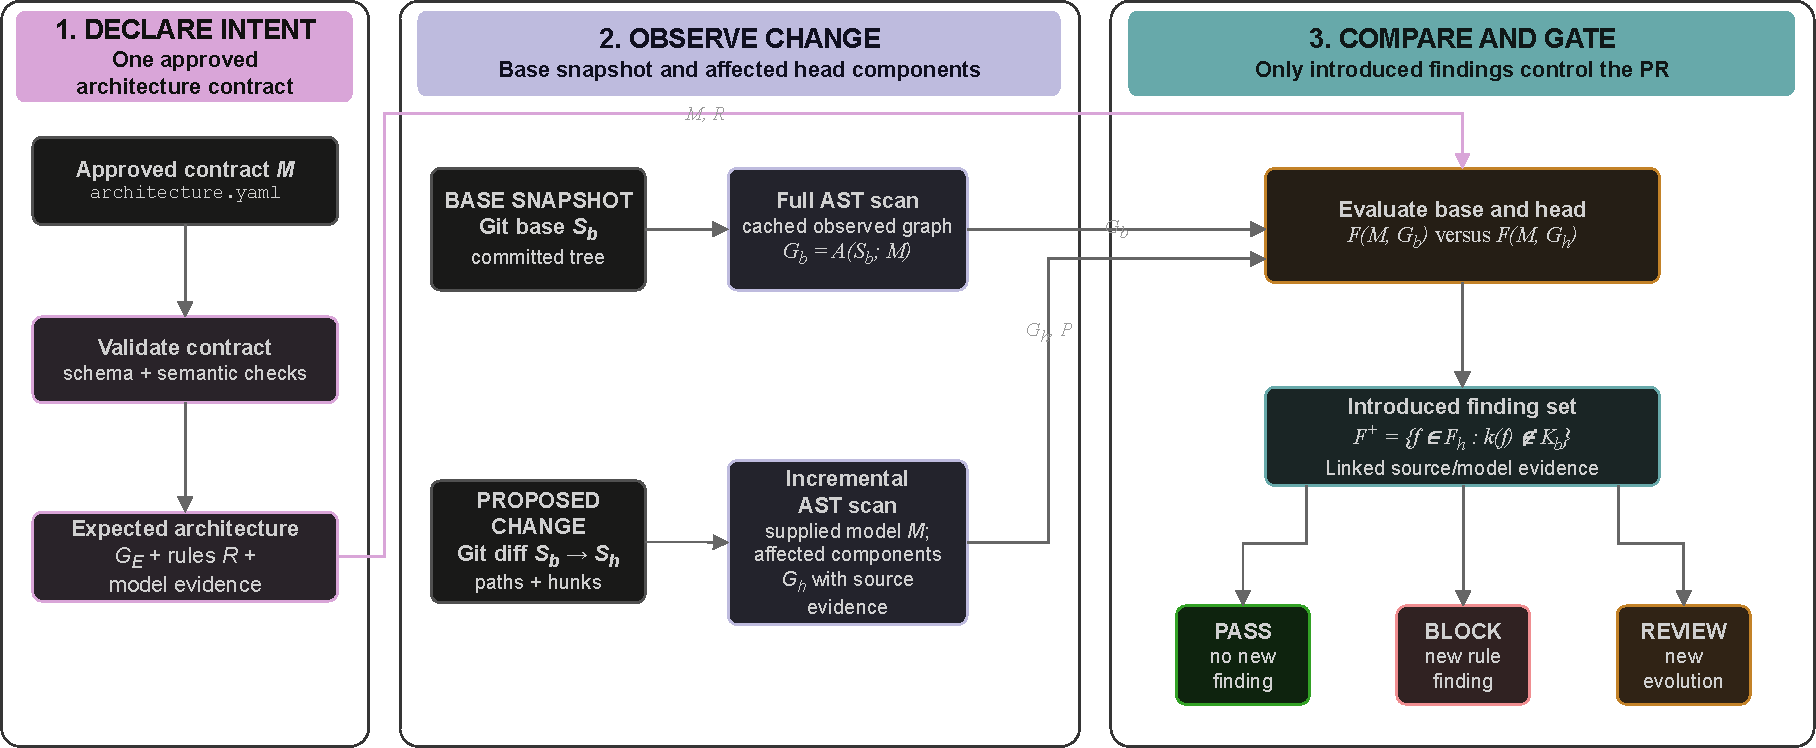
\includegraphics[width=\textwidth]{figures/Fig-1.pdf}
  \caption{ArchSync Phase 3 system architecture. The three-stage pipeline separates approved intent, base/head observation, and the pull-request gate. The model remains authoritative; only findings introduced by the Git diff determine PASS, BLOCK, or REVIEW.}
  \Description{Stage one validates the approved architecture contract into an expected graph, rules, and model evidence. Stage two builds a cached base graph and incrementally reconstructs the proposed head with source evidence. Stage three compares base and head findings, keeps the introduced set, and maps it to PASS, BLOCK, or REVIEW.}
  \label{fig:architecture}
\end{figure*}

The architecture is divided across focused repositories. \archsyncrepository{archsync-core}{https://github.com/Little-Boy-s-ArchSync/archsync-core} contains the architecture contract and deterministic conformance functions. \archsyncrepository{archsync-guardian}{https://github.com/Little-Boy-s-ArchSync/archsync-guardian} contains analyzers and findings. \archsyncrepository{archsync-benchmark}{https://github.com/Little-Boy-s-ArchSync/archsync-benchmark} contains the controlled development benchmark. \archsyncrepository{archsync-examples}{https://github.com/Little-Boy-s-ArchSync/archsync-examples} contains readable models and generated views. \archsyncrepository{archsync-mcp}{https://github.com/Little-Boy-s-ArchSync/archsync-mcp} is reserved for a later interaction layer and is excluded from the initial experiment. The named draft exposes these real repository links; the double-blind build replaces them with blinded artifact labels.
